%\documentclass[11pt,aspectratio=169]{beamer}
\documentclass[11pt,aspectratio=169,handout]{beamer}

\usetheme{Boadilla}
\usepackage[utf8]{inputenc}
\usepackage[T1]{fontenc}
\usepackage{lmodern}
\usepackage{lipsum}
\usetheme{default}
\usepackage{cancel}
\usepackage{xcolor}
\hypersetup{
	colorlinks=true,
	linkcolor=blue,
	filecolor=magenta,      
	urlcolor=cyan
}
\usepackage{amsmath}
\usepackage{listings}
\lstset{language=[90]Fortran,
	basicstyle=\small\ttfamily,
	showtabs=false,
	tabsize=2,      
	keywordstyle=\color{red},
	commentstyle=\color{green},
	morecomment=[l]{!\ }% Comment only with space after !
}

\begin{document}
	%%%%%%%%%%%%%GTA
%\renewcommand{\(}{\left(}
%\renewcommand{\)}{\right)}
%\renewcommand{\[}{\left[}
%\renewcommand{\]}{\right]}

\newcommand{\calpha}{\alpha^\ast}
\newcommand{\calphas}{\alpha^{\ast2}}
\newcommand{\Kr}[2]{\delta_{#1}^{#2}}

%%%%%%%%%%%%%%%%%%%%


\newcommand{\sqNsotwo}{\sqrt{\dfrac{Ns}{2}}}
\newcommand{\oneoNs}{\dfrac{1}{Ns}}

\let\originalleft\left
\let\originalright\right
\renewcommand{\left}{\mathopen{}\mathclose\bgroup\originalleft}
\renewcommand{\right}{\aftergroup\egroup\originalright}


\newcommand{\vect}[1]{\boldsymbol{#1}}
\renewcommand{\vec}[1]{\vect{#1}}

\makeatletter
\newcommand*\bigcdot{{\color{gray}\mathpalette\bigcdot@{1.}}}
\newcommand*\bigcdot@[2]{\mathbin{\vcenter{\hbox{\scalebox{#2}{$\m@th#1\bullet$}}}}}
\makeatother


\DeclareMathOperator*{\argmax}{argmax}
\DeclareMathOperator*{\argmin}{argmin}
\def\rme{{\rm {e}}}
\def\rmi{{\rm {i}}}
\renewcommand{\d}{{\rm {d}}}
\def\dt{{\rm {d}}t}
\def\dddt{\dfrac{\d}{\dt}}
\def\ddt{\frac{\d}{\dt}}

% \newcommand{\sgn}{\mathop{\mathrm{sgn}}}

\newcommand{\diag}{\mathrm{diag}}


\newcommand{\idhat}{\hat{\mathds{1}}}
\newcommand{\id}{\mathds{1}}
\newcommand{\idres}{\id_\mathrm{res}}
\newcommand{\idsys}{\id_\mathrm{sys}}

\newcommand{\trfrak}{\mathfrak{Tr}}
\def\tr{{\rm{Tr}}}
\newcommand{\abss}[1]{\left|#1\right|^2}
\newcommand{\mean}[1]{\left\langle #1 \right\rangle}
\newcommand{\expect}[1]{\mathbb{E}\left[ #1\right]}

%%%%%%%%%%%%%%%%%%% units
\newcommand{\micron}{\rm{\si{\micro\meter}}}


%%%%%%%%%%%%%%%%%%% Greek letters

\newcommand{\alphatil}{{\Tilde{\alpha}}}
\newcommand{\ass}{\alpha_{\mathrm{SS}}}
\newcommand{\alphass}{\alpha_\mathrm{SS}}
\newcommand{\alphahat}{\hat{\alpha}}
\newcommand{\betahat}{\hat{\beta}}
\newcommand{\betatil}{{\Tilde{\beta}}}
% \newcommand{\betatil}{\Tilde{\beta}}

\newcommand{\delhat}{\hat{\delta}}
\newcommand{\ddelhat}{\hat{\delta}^\dagger}

\newcommand{\Jhat}{\hat{J}}

\newcommand{\Lammat}{\boldsymbol{\Lambda}}

\newcommand{\lambdown}{\lambda^{\downarrow}}

\newcommand{\rhoh}{\hat{\rho}}

\newcommand{\rhohat}{\hat{\rho}}
\newcommand{\rhotil}{\tilde{\rho}}
\newcommand{\rhoss}{\rhohat_{\mathrm{SS}}}

\newcommand{\phihat}{\hat{\phi}}
\newcommand{\phidot}{\Dot{\phi}}
\newcommand{\phimat}{\vec{\Phi}}

\newcommand{\Pihat}{\hat{\Pi}}
\newcommand{\pihat}{\hat{\pi}}
\newcommand{\piit}{\mathit{\Pi}}
\newcommand{\piithat}{\hat{\piit}}

\newcommand{\psitilde}{\widetilde{\ket{\psi}}}

\newcommand{\epsvec}{\vec{\epsilon}}

\newcommand{\Obold}{\mathbf{\Omega}}

\newcommand{\Gammatil}{\Tilde{\Gamma}}

\newcommand{\sigmam}{\hat{\sigma}^{-}}
\newcommand{\sigmap}{\hat{\sigma}^{+}}
\newcommand{\sigmax}{\hat{\sigma}^{x}}
\newcommand{\sigmay}{\hat{\sigma}^{y}}
\newcommand{\sigmaz}{\hat{\sigma}^{z}}
\newcommand{\sigmamz}{\hat{\sigma}^{-z}}
\newcommand{\sigmamx}{\hat{\sigma}^{-x}}

\newcommand{\ssp}{\hat{\sigma}^+}
\newcommand{\ssm}{\hat{\sigma}^-}
\newcommand{\ssx}{\hat{\sigma}^x}
\newcommand{\ssy}{\hat{\sigma}^y}
\newcommand{\ssz}{\hat{\sigma}^z}
\newcommand{\ssa}{\hat{\sigma}^\alpha}
\newcommand{\sssz}{\hat{\sigma}^z}
\newcommand{\sigbold}{\bm{\sigma}}

\newcommand{\sigmahat}{\hat{\sigma}}

%%%%%%%%%%%%%%%% abbreviations
\newcommand{\schr}{Schr\"{o}dinger}
\newcommand{\kg}{{\mathrm{KG}}}

\newcommand{\hc}{\mathrm{H.c.}}
%\newcommand{\pv}{\mathrm{p.v.}}

\newcommand{\LP}{\mathrm{LP}}
\newcommand{\UP}{\mathrm{UP}}

%%%%%%%%%%%%%%%% Latin letters


\newcommand{\aaa}{\hat{a}}
\newcommand{\daaa}{\hat{a}^\dagger}
\newcommand{\daaas}{\hat{a}^{\dagger 2}}
\newcommand{\aaas}{\aaa^{2}}

\newcommand{\Ahat}{\hat{A}}
\newcommand{\dAhat}{\Ahat^{\dagger}}
\newcommand{\Atil}{\hat{\tilde{A}}}
\newcommand{\dAtil}{\hat{\tilde{A}}^\dagger}


\newcommand{\Avec}{\vec{A}}
\newcommand{\Avechat}{\hat{\bm{A}}}
\newcommand{\acal}{\mathcal{A}}

\newcommand{\bbb}{\hat{b}}
\newcommand{\dbbb}{\hat{b}^\dagger}
\newcommand{\bbbs}{\bbb^{2}}
\newcommand{\dbbbs}{\bbb^{\dagger 2}}

\newcommand{\BS}{\widehat{\mathrm{BS}}}

\newcommand{\bvec}{\vec{b}}

\newcommand{\Bvec}{\vec{B}}
\newcommand{\Bvechat}{\hat{\bm{B}}}

\newcommand{\Bhat}{\hat{B}}

\newcommand{\cvec}{\vec{c}}
% \newcommand{\ccal}{\mathcal{C}}
\newcommand{\ccc}{\hat{c}}
\newcommand{\dccc}{\hat{c}^\dagger}

\newcommand{\ccal}{\mathcal{C}}

\newcommand{\dcal}{\mathcal{D}}

\newcommand{\dvec}{\vec{d}}

\newcommand{\Ehat}{\hat{E}}
\newcommand{\Evec}{\vec{E}}
\newcommand{\evec}{\vec{e}}
\newcommand{\Evechat}{\hat{\bm{E}}}
\newcommand{\ecal}{\mathcal{E}}



\newcommand{\Fbold}{\mathbf{F}}

\newcommand{\fhat}{\hat{f}}
\newcommand{\fcal}{\mathcal{F}}
\newcommand{\gcal}{\mathcal{G}}
\newcommand{\Gmat}{\boldsymbol{\mathrm{G}}}

% \newcommand{\Ehat}{\hat{E}}
\newcommand{\ecalf}{\ecal^{F}}

\newcommand{\ecalu}{\ecal^{U}}
\newcommand{\fcalu}{\fcal^{U}}
\newcommand{\czu}{\ccal_{\ztil}^{U}}

\newcommand{\ecaluc}{\ecal^{U*}}
\newcommand{\fcaluc}{\fcal^{U*}}
\newcommand{\czuc}{\ccal_{\ztil}^{U*}}

\newcommand{\ecald}{\ecal^{D}}
\newcommand{\fcald}{\fcal^{D}}
\newcommand{\czd}{\ccal_{\ztil}^{D}}

\newcommand{\ecaldc}{\ecal^{D*}}
\newcommand{\fcaldc}{\fcal^{D*}}
\newcommand{\czdc}{\ccal_{\ztil}^{D*}}

\newcommand{\ecali}{\ecal^{I}}
\newcommand{\fcali}{\fcal^{I}}
\newcommand{\czi}{\ccal_{\ztil}^{I}}

\newcommand{\ecalic}{\ecal^{I*}}
\newcommand{\fcalic}{\fcal^{I*}}
\newcommand{\czic}{\ccal_{\ztil}^{I*}}


\newcommand{\hcal}{\mathcal{H}}
\newcommand{\hh}{\hat{H}}
\newcommand{\heff}{\hat{H}_\text{eff}}

\newcommand{\Hhat}{\hat{H}}
\newcommand{\hhat}{\hat{h}}
\newcommand{\htil}{\tilde{H}}

\newcommand{\Khat}{\hat{K}}
\newcommand{\kvec}{{\vec{k}}}


\newcommand{\lio}{\mathcal{L}}
\newcommand{\liou}{\mathcal{L}}
\newcommand{\Liou}{\liou}

\newcommand{\lioeff}{\mathcal{L}_\text{eff}}

\newcommand{\lcal}{\mathcal{L}}
\newcommand{\Lhat}{\hat{L}}
\newcommand{\Ltil}{\tilde{L}}
\newcommand{\Lcal}{\mathcal{L}}

\newcommand{\mev}{\mathrm{meV}}


\newcommand{\mcal}{\mathcal{M}}

\newcommand{\mvec}{{\vec{m}}}
\newcommand{\nsys}{{N_\mathrm{sys}}}
\newcommand{\nres}{{N_\mathrm{res}}}

\newcommand{\ncal}{\mathcal{N}}

\newcommand{\nvec}{{\vec{n}}}

\newcommand{\ohat}{\hat{O}}
\newcommand{\otil}{\tilde{O}}
\newcommand{\ovec}{{\vec{0}}}
\newcommand{\ocal}{\mathcal{O}}

\newcommand{\Ohat}{\hat{O}}

\newcommand{\phat}{\hat{p}}
\newcommand{\pvec}{\vec{p}}
\newcommand{\pcal}{\mathcal{P}}
\newcommand{\pscr}{{\mathscr{P}}}

\newcommand{\qdot}{\dot{q}}
\newcommand{\qhat}{\hat{q}}
\newcommand{\qvec}{\vec{q}}
\newcommand{\qcal}{\mathcal{Q}}
\newcommand{\Rhat}{\hat{R}}
\newcommand{\Rtil}{\tilde{R}}

\newcommand{\R}{\mathbb{R}}

\newcommand{\rvec}{\vec{r}}
\newcommand{\res}{\mathrm{res}}

\newcommand{\rf}{{\mathrm{RF}}}

\newcommand{\Shat}{\hat{S}}
\newcommand{\shat}{\hat{s}}
\newcommand{\svec}{\hat{\vec{\sigma}}}
\newcommand{\sys}{\mathrm{sys}}

\newcommand{\Svec}{\vec{S}}
\newcommand{\Stil}{\tilde{S}}
\newcommand{\Sbold}{\mathbf{S}}
\newcommand{\scal}{\mathcal{S}}

\newcommand{\tcal}{\mathcal{T}}

\newcommand{\Uhat}{\uhat}
\newcommand{\uhat}{\hat{U}}
\newcommand{\udag}{\hat{U}^\dagger}
\newcommand{\Umat}{\boldsymbol{\mathrm{U}}}
\newcommand{\uvec}{\vec{u}}

\newcommand{\ua}{u^{(a)}}
\newcommand{\uac}{u^{(a)*}}
\newcommand{\uab}{u^{(ab)}}
\newcommand{\uabc}{u^{(ab)*}}
\newcommand{\ub}{u^{(b)}}
\newcommand{\ubc}{u^{(b)*}}




\newcommand{\delhata}{\hat{\delta}^{(a)}}
\newcommand{\delhatb}{\hat{\delta}^{(b)}}

\newcommand{\ddelhata}{\hat{\delta}^{(a)\dagger}}
\newcommand{\ddelhatb}{\hat{\delta}^{(b)\dagger}}

\newcommand{\wvec}{\vec{w}}

\newcommand{\xhat}{\hat{x}}

\newcommand{\xvec}{\vec{x}}
\newcommand{\xmu}{x^{\mu}}
\newcommand{\xpmu}{x^{\prime\mu}}
\newcommand{\xnu}{x^{\nu}}
\newcommand{\xpnu}{x^{\prime\nu}}

\newcommand{\rmx}{\mathrm{x}}
\newcommand{\xvecrm}{\vec{\mathrm{x}}}
\newcommand{\rmxvec}{\xvecrm}
\newcommand{\Xvec}{\vec{X}}
\newcommand{\xcal}{\mathcal{X}}

\newcommand{\xtil}{{\Tilde{x}}}

\newcommand{\yvec}{\vec{y}}
\newcommand{\ycal}{\mathcal{Y}}
\newcommand{\ytil}{{\Tilde{y}}}

\newcommand{\Vhat}{\hat{V}}
\newcommand{\ztil}{{\Tilde{z}}}
\newcommand{\z}{\mathbb{Z}}
\newcommand{\zerovec}{\vec{0}}
\newcommand{\zvec}{{\vec{z}}}

\newcommand{\zcal}{\mathcal{Z}}
% \renewcommand{\ket}[1]{|#1\rangle}

\newcommand{\pmx}[1]{\begin{pmatrix}
		#1
\end{pmatrix}}


\newcommand{\bea}{\begin{equation*}\begin{aligned}}
		\newcommand{\eea}{\end{aligned}\end{equation*}}
\newcommand{\be}{\begin{equation*}}
	\newcommand{\ee}{\end{equation*}}

\newcommand{\redtext}[1]{\textcolor{red}{#1}}
\author{Zejian Li \\(li.zejian@ictp.it)}
\title{Lecture 2-3: Differential Equations (II)}
%\logo{}
%\institute{}
\date{25. Oct. 2023}
%\subject{}
%\setbeamercovered{transparent}
%\setbeamertemplate{navigation symbols}{}


% ----------------------------------------------------------------
\begin{frame}[plain]
	\maketitle
\end{frame}


% ----------------------------------------------------------------
\begin{frame}
\frametitle{Last lecture}

\begin{itemize}
	\item Euler \& midpoint methosd for 1st order ODEs.
\end{itemize}
\begin{figure}
	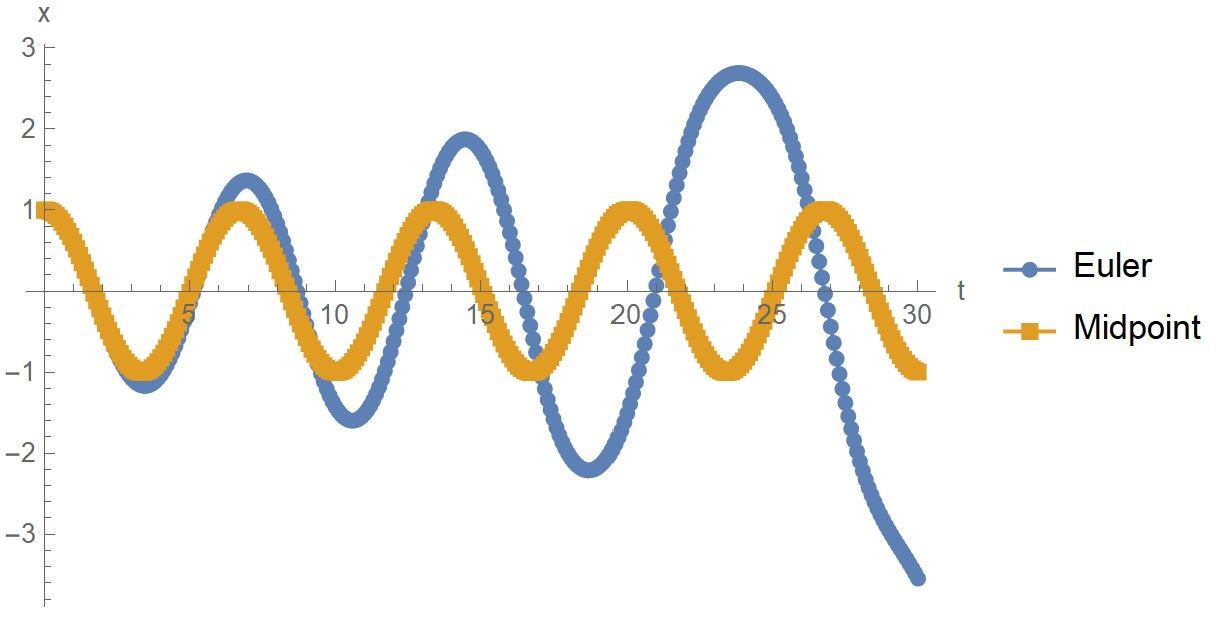
\includegraphics[width=0.7\textwidth]{fig/euler-vs-mid}
\end{figure}
\begin{center}
	Solution to $\dfrac{\mathrm{d}^2 x}{\mathrm{d}t^2} = -\sin(x)$ with (a large) \texttt{dt = 0.1}.
\end{center}
\end{frame}

\begin{frame}{Today: Verlet method for integrating Newton's equations}
	Newton's equations for conservative system (where forces only depend on positions):
	\bea
		m_i \dfrac{\d^2 \vec{x}_i}{\d t^2} = -\vec{\nabla}_{\vec{x}_i}V(\{\vec{x}_j\}_j)\equiv \vec{F}_i(\{\vec{x}_j\}_j)\,,
	\eea
	for particles with masses $m_i$ at positions $\vec{x}_i$ and interacting via the potential $V(\vec{x}_1,\cdots,\vec{x}_N)$.\\
	For example,\pause
	\begin{itemize}[<+->]
		\item Harmonic oscillator: $V(x) = \dfrac{1}{2}\omega^2 x^2$;
		\item Newtonian gravity: $V({\vec{x}_i}) = -\dfrac{1}{2}\sum_{i\neq j} \dfrac{G m_i m_j}{| \vec{x}_i - \vec{x}_j |}$
		\item Molecular potential
	\end{itemize}
\end{frame}

\begin{frame}{Today: Verlet method for integrating Newton's equations}
		Generic form of the equation:
	\bea
	\dfrac{\d^2 \vec{x}(t)}{\d t^2} = \vec{a}[\vec{x}(t)]\,.
	\eea\pause
	Idea of the algorithm:\pause
	\begin{itemize}[<+->]
		\item Evolve velocity for half a step: 
		\bea
			\vec{v}\left(t+\dfrac{1}{2}\Delta t\right) \simeq \vec{v}(t) + \dfrac{1}{2}\vec{a}[\vec{x}(t)] \Delta t\,.
		\eea
		\item Evolve position for a full step using the mid-point velocity:
		\bea
			\vec{x}(t+\Delta t) \simeq \vec{x}(t) + \vec{v}\left(t+\dfrac{1}{2}\Delta\right)\Delta t\,.
		\eea
		\item Evolve velocity for another half step using acceleration at updated position:
		\bea
			\vec{v}(t+\Delta t) \simeq 	\vec{v}\left(t+\dfrac{1}{2}\Delta t\right) + \dfrac{1}{2}\vec{a}[\vec{x}(t+\Delta t)]\Delta t\,.
		\eea
	\end{itemize}
\end{frame}

\begin{frame}{In case you wonder why ...}\pause
	Suppose (for a single particle in 1D) we want to find the dynamics of a function $\phi(t)\equiv \phi[x(t), p(t)]$ depending only on position $x$ and momentum $p = mv$.\pause\\
	One get from Hamiltonian mechanics:
	\bea
		\phi(t) = \rme^{\rmi \lcal t}\phi(0)\,,\quad \rmi\lcal(\bigcdot) = \dfrac{p}{m}\cdot\dfrac{\partial(\bigcdot)}{\partial x} + F\cdot\dfrac{\partial(\bigcdot)}{\partial p}\,.
	\eea\pause
	\begin{itemize}[<+->]
		\item The generator has two non-commuting parts: 
		\bea
			\rmi\lcal = \rmi\lcal_1 + \rmi\lcal_2\,,\quad\rmi\lcal_1(\bigcdot)\equiv\dfrac{p}{m}\cdot\dfrac{\partial(\bigcdot)}{\partial x}\,,\quad\rmi\lcal_2(\bigcdot)\equiv F\cdot\dfrac{\partial(\bigcdot)}{\partial p}\,,\quad [\rmi\lcal_1,\rmi\lcal_2]\neq 0\,.
		\eea
		\item \href{https://www.jstor.org/stable/2033649?seq=7}{Trotter theorm (1959)} implies:
		\bea
			\rme^{\rmi\lcal\Delta t} = \rme^{\rmi\lcal_2\Delta t/2}\cdot\rme^{\rmi\lcal_1\Delta t}\cdot\rme^{\rmi\lcal_2\Delta t/2} + \ocal(\Delta t^3)\,.
		\eea
		\item Read more here --- \href{https://doi.org/10.1063/1.463137}{Reversible multiple time scale molecular dynamics }.
	\end{itemize}
\end{frame}

\begin{frame}
\frametitle{Verlet Method: summary}

\begin{columns}[c]
	\column{0.6\textwidth}


\begin{block}{Algorithm: velocity-Verlet Method}
	\pause
	\textbf{Input}: acceleration function $\vec{a}(\vec{x})$, initial values $t_0$, $\vec{x}_0$, $\vec{v}_0$ step size $\Delta t$, and final time $t_f$. 
	\pause
	\begin{enumerate}
		\item set $t=t_0$, $\vec{x}=\vec{x}_0$, $\vec{v}=\vec{v}_0$. 
	
		\item repeat $N = \lceil (t_f-t_0)/\Delta t\rceil$ times:
		\pause
		\begin{itemize}
			\item set $\vec{v} = \vec{v} + \vec{a}(\vec{x})\Delta t / 2$,
			\pause
			\item set $\vec{x} = \vec{x} + \vec{v}\Delta t$,
			\pause
			\item set  $\vec{v} = \vec{v} + \vec{a}(\vec{x})\Delta t / 2$.
		\end{itemize}		
	\end{enumerate}  
	\pause
	\textbf{Output}: the sequence of $t$, $\vec{x}$ and $\vec{v}$ approximating the solution of $\frac{\d^2 \vec{x}}{\d t^2} = \vec{a}(\vec{x})$.
\end{block}
\column{0.3\textwidth}
\pause
\begin{alertblock}{Comparison with Euler method}
	\pause
	\textbf{Input}: Same as left
	\pause
	\begin{enumerate}
		\item Same as left
		
		\item repeat $N$ times:
		\pause
		\begin{itemize}
			\item set $\vec{a}_t = \vec{a}(\vec{x})$,
			\pause
			\item set $\vec{x} = \vec{x} + \vec{v}\Delta t$,
			\pause
			\item set  $\vec{v} = \vec{v} + \vec{a}_t\Delta t$.
		\end{itemize}		
	\end{enumerate}  
	\pause
%	\vspace{0.5cm}
	\textbf{Output}: the sequence of $t$, $\vec{x}$ and $\vec{v}$.
\end{alertblock}

\end{columns}
\vspace{0.4cm}
\begin{itemize}
	\item Good numerical stability and other important physical properties: time reversibility and preservation of the symplectic form on phase space, at no significant additional computational cost over the simple Euler method.
\end{itemize}
\end{frame}


\begin{frame}
\frametitle{Assignment 13}
Write a \texttt{Fortran} program that solves the equation of motion for a frictionless physical pendulum (again) using the velocity-Verlet method: $\frac{\d^2 x}{\d t^2} = -\sin(x)\,.$

\pause
\begin{itemize}
	\item You can base your program on the previous assignment (hint: see the comparison on the previous slide).
	\item Solve with the initial conditions \texttt{t0=0, x0=1.0, v0=0.0} and \texttt{dt = 0.1, tf=30}.
	\item The program should create a file (\texttt{verlet.txt}) with the result in three columns: \texttt{t}, \texttt{x(t)} and \texttt{v(t)}.\pause
	\item Plot the result $x$ versus $t$ with your favorite plotting program.\pause
\end{itemize}
\textbf{Bonus question:}
\begin{itemize}
	\item Expand your subroutines and solve the equation of motion for a point mass in a gravitational field (moving in a 2D plane): $\frac{\mathrm{d}^2 \vec{x}}{\mathrm{d} t^2} = -\vec{x}/|\vec{x}|^3$ using the Euler and verlet methods, with initial conditions \texttt{t0=0, x0=(/2.0, 0.0/),  v0 = (/0.0, 0.5/)} and \texttt{dt = 0.1, tf=30}. Plot the trajectory [ $x(1)$ vs $x(2)$ ] and compare the performance between the two methods.
\end{itemize}
Submit the graphs and your code as \texttt{Ass13.YourLastName.f90} to \texttt{li.zejian@ictp.it} before the next lesson.
\end{frame}

\end{document}